% Quick start guide
\documentclass{beamer}
\usepackage{bookmark}
\usepackage{xeCJK}  % 使用中文字体
\usepackage{tikz}   % 为了首页的背景图片
\usepackage{graphicx}

\usefonttheme[onlymath]{serif}


% Title Page Details
\title{近期工作情况汇报}
\subtitle{BFU::Tech::FEIA Lab}
\author{Jiaming Zhang}
\institute[BFU::Tech]{北京林业大学-工学院}
\date{\today}

\begin{document}
% ==============================================================
% ===================== 标题页帧 ================================
% ==============================================================
{  % 校徽、校名、建筑物
    \usebackgroundtemplate{
        \tikz[overlay, remember picture]
        \node[opacity=0.4] at (
                0.5\paperwidth, 
                30-\paperheight){
            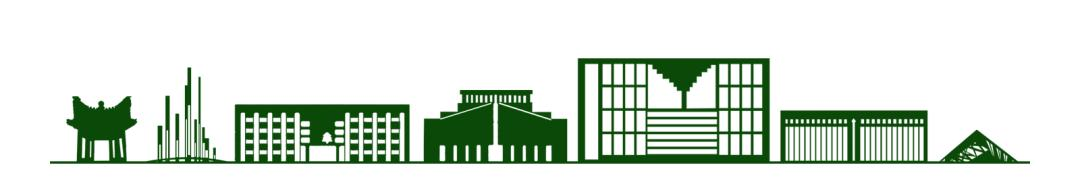
\includegraphics[width=0.7\paperwidth]{
                template_pics/buildings
                }
            };
        \tikz[overlay, remember picture]
        \node[opacity=0.8] at (
                0.5\paperwidth, 
                240-\paperheight){
            
\includegraphics[width=0.5\paperwidth]{
                template_pics/logo_name
                }
            };
    }
    % 标题页帧
    \begin{frame}
        \titlepage
    \end{frame}
}  % 校徽、校名、建筑物

% ==============================================================
% ===================== 目录页帧 ================================
% ==============================================================
{  % 用于半透明黑色北林logo
    % 目录页背景
    \usebackgroundtemplate{
        \tikz[overlay, remember picture]
        \node[opacity=0.1]at (0, 145-\paperheight){
            
\includegraphics[width=\paperwidth]{
                template_pics/logo_black
                }
            };
    }
    % 目录
    \begin{frame}\frametitle{Outline}
        \tableofcontents% [hideallsubsections]
            % 可选参数:
            % part=数字 显示指定的篇目录;
            % currentsection 除了其它节都以半透明的方式显示;
            % hideothersubsections 只显示当前小节;
            % hideallsubsections 隐藏所有的小节
            % firstsection=数字 指明哪一节开始才是第一节;
        \end{frame}
}  % 用于半透明黑色北林logo
{  % 用于北林校名+英文边框
% 引入边框
\usebackgroundtemplate{
        \tikz[overlay, remember picture]
        \node[opacity=1]at 
            (0.13, -0.505\paperheight){
            
\includegraphics[
                height=\paperheight, 
                width=0.02\paperwidth]{
                    template_pics/edge
                    }
            };
    }

% ==============================================================
% ===================== 正文开始! ===============================
% ==============================================================
% 如何添加新的幻灯片?
% \section{数学测试}
%   \subsection{测试}
%   \begin{frame}\frametitle{测试}
%       ...Contents...

\section{数学测试}
    \subsection{测试}
    \begin{frame}\frametitle{测试}
        Something \pause % pause 命令让后面的东西在下一页展示

        $x^n+y^n=z^n$
    \end{frame}

    \subsection{分层规格}
    \begin{frame} 

        下面我们要证明没有最大的质数。
    
        \begin{itemize}
            \item<1-> x- 表示从第 xx 张开始显示。可以描述为区间 [x,n][x,n] n 是该帧所需的幻灯片张数。
            \item<3-> -x 表示在第 xx 张以前显示。可以描述为区间 [1,x][1,x]。
            \item<1-> x-y 表示从第 xx 张开始显示,到第 yy 张结束,其中 $x\le y$。可以描述为区间 [x,y][x,y]。
            \item<2-> 这是一个测试哦,以上 3 种混合使用,用 \\texttt,, 隔开。可以描述为组成各部分的并集。
        \end{itemize}
    
    \end{frame}

\section{介绍}
    \subsection{历史}
    \begin{frame} \frametitle{历史}
        This is your first presentation!
    \end{frame}


% ==============================================================
% ===================== 正文结束! ===============================
% ==============================================================

} % 用于北林校名+英文边框
\end{document}